\subsubsection{Secure Element} \label{section:counter-replace-encryption-key-local}
Since there is the possibility to read the cached encryption key \cite{memoryDump} and crack the encryption, the use of \gls{se} is proposed.
A secure element is a tamper-resistant platform which can be used to securely host applications and cryptographic keys \cite{seDefinition}.
There are different form factors for \gls{se}s.
For Android, the microSD form factor is the interesting one.
It can be either mounted in the microSD card slot or by using an adapter on the USB interface, which requires the device to support \gls{otg} \cite{usbOtg}.
The resource is accessed over reads and writes to the filesystem.
Since the \gls{se} has to be small to fit the size of an microSD card and powered by the host system, its hardware capabilities are constrained.
The result is a performance of 25MHz which does not allow complexe comnputations. \cite{stSe}
\newline
For this reason the usage of the \gls{se} is restricted to simple tasks, like storing a key used for decryption.
The advantage of an \gls{se} is that its functionality is outside of the Android application and thus cannot be manipulated by \gls{luckypatcherg}.
\newline
An abstract presentation of the use of a \gls{se} can be seen in figure~\ref{fig:encryptionKeySmart}.
\newline
\begin{figure}[h]
    \centering
    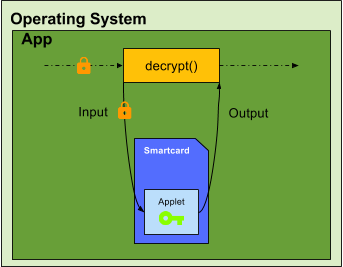
\includegraphics[width=0.8\textwidth]{data/encryptionKeySmart.png}
    \caption{Decryption by using a smartcard}
    \label{fig:encryptionKeySmart}
\end{figure}
Integrating a \gls{se} comes with some problems.
\begin{itemize}
  \item the user has to buy extra hardware
  \item not all devices have a microSD card slot or support \gls{otg}
  \item different implementations for communication with the \gls{se}
\end{itemize}
The first problem is that the user is required to buy extra hardware.
This means the user has to spend extra cache and to have the \gls{se} always around.
The connection to the device using a cable is not the most convenient solution as well.
The second problem is that not all devices either have an microSD card slot, nor \gls{otg} support.
For example, the Nexus 7 (2012) and the Nexus 6P neither have the capability to use a microSD card.
While the Nexus7 was supposed to have \gls{otg}, it did not work with the used \gls{se}, while the Nexus 6P did not support \gls{otg} out of the box.
Both devices needed even needed additional plugins to read the \gls{otg} mounted microSD in a file explorer.
The third problem is that each manufacturer implements its own interpretation for the interface which makes \gls{se} incompatible to each other.
For this reason, the SD Association proposed the smartSD in order to have a universal standard for \gls{se}s \cite{smartSD}.
\newline


se signiert mit key+android\_id welche unique ist

TODO:
2) Secure Elements
Bottleneck ist sicherlich die Schnittstelle zu Android und alles was in Android ist, ist prinzipiell unsicher, also auch etwaige Keys. Was jedoch koennte Secure Elements absichern? Ich moechte dich bitten hier Ideen zu erarbeiten, was im Zuge von Kopierschutz,  Verschluesslung etc. mit SEs wirklich sicher gemacht werden koennte. Eine grobe Idee ist z.B. das Signieren von Serveranfragen. Key kennt hier nur das SE und der Server. Android schickt die volle URL mit Parametern und das SE fuegt einen Signaturparameter zu. Vorteil: Ohne das SE kann die App den Server mal nicht mehr nutzen. Jetzt musste man verhindern, dass eine Proxy-App unter Android fuer andere aktiv wird (Stichwort CardSharing). Was koennte man tun? Das ist auch nur ein Idee. Was gibt es sonst noch? Wo koennte es Sinn machen einen sicheren Speicher zu haben?
